% Gabarit pandoc des corrigés publiés (brut et guidé). Contenu sans marque ni nom de site.
% Compilation : lualatex (latexmk -lualatex).
% Le Markdown reste la source unique : ne pas éditer ce fichier .tex à la main.
\documentclass[11pt,a4paper]{article}

% --- Moteur, polices (Latin Modern) et langue ---------------------------------
\usepackage{iftex}
\ifLuaTeX\else\errmessage{Ce document se compile avec lualatex}\fi
\usepackage{amsmath,amssymb,mathtools}
\usepackage{fontspec}
% mathrm=sym : \mathrm prend ses glyphes dans la police mathématique (ℓ, μ, Ω), comme KaTeX.
\usepackage[math-style=TeX,bold-style=TeX,mathrm=sym]{unicode-math}
% Repli pour les glyphes absents de Latin Modern (indices et exposants Unicode,
% flèches, filets des schémas en texte, symboles) : DejaVu, puis Latin Modern Math
% (ℓ, lettres mathématiques Unicode des légendes).
\directlua{
  luaotfload.add_fallback("repliTexte", {"DejaVuSerif:mode=harf;", "DejaVuSans:mode=harf;", "file:latinmodern-math.otf:mode=harf;"})
  luaotfload.add_fallback("repliMono", {"DejaVuSansMono:mode=harf;", "DejaVuSans:mode=harf;", "file:latinmodern-math.otf:mode=harf;"})
}
\setmainfont{Latin Modern Roman}[RawFeature={fallback=repliTexte}]
\setsansfont{Latin Modern Sans}[RawFeature={fallback=repliTexte}]
\setmonofont{Latin Modern Mono}[RawFeature={fallback=repliMono}]
\setmathfont{Latin Modern Math}
\usepackage[french]{babel}
\frenchsetup{SmallCapsFigTabCaptions=false}

% --- Mise en page --------------------------------------------------------------
\usepackage[a4paper,margin=2.2cm,headheight=14pt,footskip=1.2cm]{geometry}
\usepackage{microtype}
\setlength{\emergencystretch}{4em}
\tolerance=1500
\setlength{\parindent}{0pt}
\setlength{\parskip}{0.55\baselineskip plus 2pt minus 1pt}
\usepackage{xcolor}
% Gris nommés : babel-french rend « ! » actif dans le document.
\definecolor{gris2}{gray}{0.98}
\definecolor{gris3}{gray}{0.97}
\definecolor{gris5}{gray}{0.95}
\definecolor{gris35}{gray}{0.65}
\definecolor{gris40}{gray}{0.60}
\definecolor{gris45}{gray}{0.55}
\definecolor{gris50}{gray}{0.50}
\definecolor{gris55}{gray}{0.45}
\definecolor{gris60}{gray}{0.40}
\definecolor{gris65}{gray}{0.35}
\definecolor{gris70}{gray}{0.30}
\definecolor{gris80}{gray}{0.20}
\definecolor{gris85}{gray}{0.15}
\usepackage{graphicx}
\usepackage{float}
\usepackage{caption}
\captionsetup{font=small,labelformat=empty,justification=centering}
\usepackage{booktabs,longtable,array,multirow,calc}
\usepackage{siunitx}
\sisetup{locale=FR}
\usepackage[version=4]{mhchem}
\usepackage{listings}
\usepackage{fancyhdr}
\usepackage{lastpage}
\usepackage[most]{tcolorbox}
\usepackage{enumitem}
\setlist{nosep,leftmargin=*,topsep=2pt}
\usepackage[hidelinks,unicode]{hyperref}
\usepackage{bookmark}
\hypersetup{pdftitle={CCINP MP — Mathématiques 2 2026},pdfauthor={Rédigé par IA},pdfcreator={LaTeX},pdfsubject={Corrigé guidé}}
\usepackage{xurl}

% --- Pandoc : listes, tableaux, figures ----------------------------------------
\providecommand{\passthrough}[1]{#1}
\providecommand{\tightlist}{\setlength{\itemsep}{0pt}\setlength{\parskip}{0pt}}

\makeatletter
\def\maxwidth{\ifdim\Gin@nat@width>\linewidth\linewidth\else\Gin@nat@width\fi}
\def\maxheight{\ifdim\Gin@nat@height>0.55\textheight 0.55\textheight\else\Gin@nat@height\fi}
\makeatother
\setkeys{Gin}{width=\maxwidth,height=\maxheight,keepaspectratio}
\setcounter{secnumdepth}{-\maxdimen}
\providecommand{\pandocbounded}[1]{#1}

% --- Code (listings) -----------------------------------------------------------
\lstset{
  basicstyle=\ttfamily\small,
  columns=fullflexible,
  keepspaces=true,
  breaklines=true,
  breakatwhitespace=false,
  postbreak=\mbox{\textcolor{gris50}{$\hookrightarrow$}\space},
  frame=single,
  rulecolor=\color{gris35},
  framesep=4pt,
  xleftmargin=5pt,xrightmargin=5pt,
  backgroundcolor=\color{gris3},
  keywordstyle=\bfseries,
  commentstyle=\color{gris65},
  stringstyle=\color{gris80},
  showstringspaces=false,
  tabsize=4,
  extendedchars=true,
  aboveskip=6pt,belowskip=6pt,
}

% --- Macros des corrigés (KaTeX ↔ LaTeX) ---------------------------------------
% Les corrigés sont écrits pour KaTeX : on définit ici ce que KaTeX connaît et
% que LaTeX n'a pas, sans jamais retoucher le Markdown.
\providecommand{\R}{\mathbb{R}}
\providecommand{\N}{\mathbb{N}}
\providecommand{\Z}{\mathbb{Z}}
\providecommand{\Q}{\mathbb{Q}}
\providecommand{\C}{\mathbb{C}}
\providecommand{\dd}{\mathrm{d}}
\providecommand{\llbracket}{\lBrack}
\providecommand{\rrbracket}{\rBrack}
\providecommand{\lBrace}{\lbrace}
\providecommand{\rBrace}{\rbrace}
\providecommand{\Box}{\square}
\providecommand{\Diamond}{\lozenge}
\providecommand{\varnothing}{\emptyset}
\providecommand{\argmax}{\operatorname*{arg\,max}}
\providecommand{\argmin}{\operatorname*{arg\,min}}
\renewcommand{\leq}{\leqslant}
\renewcommand{\geq}{\geqslant}

% Équation hors texte : réduite à la largeur de la ligne si elle déborde.
\newsavebox{\boiteequation}
\newcommand{\equationajustee}[1]{%
  \sbox{\boiteequation}{$\displaystyle #1$}%
  \ifdim\wd\boiteequation>\linewidth
    \[\resizebox{\linewidth}{!}{\usebox{\boiteequation}}\]%
  \else
    \[#1\]%
  \fi}

% --- Encadrés pédagogiques (sobres, lisibles en noir et blanc) -----------------
\tcbset{
  encadre/.style={
    enhanced,breakable,sharp corners,
    colback=white,colframe=gris55,
    boxrule=0.4pt,leftrule=2.2pt,
    left=6pt,right=6pt,top=3pt,bottom=3pt,
    before skip=6pt,after skip=6pt,
    fonttitle=\bfseries\small,coltitle=black,
    attach title to upper,after title={\quad},
    parbox=false,
  }
}
\newtcolorbox{indication}[1]{encadre,colframe=gris45,colback=gris2,title={Indication~#1}}
\newtcolorbox{methode}{encadre,colframe=gris70,title={Méthode}}
\newtcolorbox{piege}{encadre,colframe=gris85,boxrule=0.8pt,leftrule=2.2pt,title={Piège}}
\newtcolorbox{jury}{encadre,colframe=gris60,colback=gris5,title={Jury}}
\newtcolorbox{encadrenote}{encadre,colframe=gris40}

% --- Titres de section ---------------------------------------------------------
\usepackage{titlesec}
\titleformat{\section}{\Large\bfseries}{}{0pt}{}
\titleformat{\subsection}{\large\bfseries}{}{0pt}{}
\titleformat{\subsubsection}{\normalsize\bfseries}{}{0pt}{}
\titlespacing*{\section}{0pt}{14pt plus 4pt minus 2pt}{6pt}
\titlespacing*{\subsection}{0pt}{10pt plus 3pt minus 2pt}{4pt}
\titlespacing*{\subsubsection}{0pt}{8pt plus 2pt minus 2pt}{2pt}

% --- En-tête et pied de page ---------------------------------------------------
\pagestyle{fancy}
\fancyhf{}
\fancyhead[L]{\small\textsc{Corrigé guidé} · CCINP MP}
\fancyhead[R]{\small Maths 2 2026}
\fancyfoot[L]{\footnotesize Corrigé rédigé par IA, non officiel}
\fancyfoot[R]{\footnotesize \thepage\,/\,\pageref*{LastPage}}
\renewcommand{\headrulewidth}{0.4pt}
\renewcommand{\footrulewidth}{0pt}
\fancypagestyle{plain}{\fancyhf{}\fancyfoot[R]{\footnotesize \thepage\,/\,\pageref*{LastPage}}\fancyfoot[L]{\footnotesize Corrigé rédigé par IA, non officiel}\renewcommand{\headrulewidth}{0pt}}

\begin{document}
\thispagestyle{plain}
\begin{center}
  {\small\scshape Corrigé guidé}\par\smallskip
  {\LARGE\bfseries CCINP MP — Mathématiques 2 2026\par}\medskip
  {\large CCINP · MP · Maths 2 · 2026\par}
\end{center}
\vspace{2pt}\hrule\vspace{8pt}

\emph{Corrigé rédigé par IA, non officiel. Signalez toute erreur.}

\hypertarget{pruxe9sentation-du-sujet}{%
\section{Présentation du sujet}\label{pruxe9sentation-du-sujet}}

\textbf{Cadre.} Épreuve MP3M2, 4 heures, calculatrices interdites. Le sujet comprend deux exercices et un problème indépendants, soit 20 questions (Q1 à Q20, dont Q4, Q10 et Q14 en deux parties).

\textbf{Exercice 1 (Q1--Q4) : réduction d'une matrice \(3\times3\).} On étudie \(A=aJ+bI_3\), où \(J\) a tous ses coefficients égaux à \(1\).

On diagonalise \(J\) sans déterminant (polynôme annulateur), on en déduit la réduction de \(A\) et son polynôme minimal. On calcule enfin \(A^n\) de deux façons : reste de la division euclidienne de \(X^n\) par \(\pi_A\), puis binôme de Newton.

\textbf{Exercice 2 (Q5--Q9) : matrices circulantes.} \(J\) est la matrice de la permutation circulaire, \(A=P(J)\) la matrice circulante associée au polynôme réel \(P\).

On calcule \(\chi_J=X^n-1\), on diagonalise \(J\) puis \(A\) dans \(\mathcal M_n(\mathbb C)\), avec pour valeurs propres les \(P(\omega_k)\). On montre enfin que \(P(\omega_1)\cdots P(\omega_{n-1})\) est réel.

\textbf{Problème (Q10--Q20) : polynômes de Laguerre.} Après une question de cours (projection orthogonale, inégalité de Bessel), on construit l'espace préhilbertien \(E\) des fonctions continues sur \([0,+\infty[\) de carré intégrable pour le poids \(\mathrm e^{-t}\).

On définit les polynômes de Laguerre par une formule de Rodrigues et l'on montre, par intégrations par parties, qu'ils forment une famille orthonormale. On obtient l'inégalité de Bessel, puis on vérifie l'égalité pour les fonctions \(g_\alpha(x)=\mathrm e^{-\alpha x}\).

\textbf{Notions mobilisées.} Polynôme annulateur et critère de diagonalisabilité, polynôme minimal, division euclidienne, binôme dans une algèbre commutative ; déterminant par développement, racines de l'unité ; espaces préhilbertiens, projection orthogonale, intégrabilité par comparaison, fonction continue positive d'intégrale nulle, formule de Leibniz, intégration par parties sur un intervalle non borné, séries à termes positifs, série géométrique.

\textbf{Difficulté et longueur.} Sujet classique, de longueur raisonnable, très guidé. Le rapport 2026 donne une moyenne de 10,18 sur 20, avec un écart-type de 4,51.

Les deux exercices sont proches du cours ; le problème demande surtout de la rigueur (intégrabilité, termes de bord). Deux points demandent du recul : le cas \(P(1)=0\) en Q9, et les défauts d'énoncé en Q15 et Q20.

En Q15, le jury a reconnu l'erreur d'énoncé et adapté le barème. En Q20, « pour tout \(\alpha\in\mathbb R\) » est faux. Dans les deux cas, il faut le signaler sur la copie et expliquer l'initiative prise.

\textbf{Questions discriminantes.} D'après le rapport 2026, les points se sont joués sur :

\begin{itemize}
\tightlist
\item
  les justifications « sans calcul » de l'exercice 1 : diagonalisabilité en Q1, caractère scindé à racines simples en Q3 ;
\item
  Q4.a, rarement abordée ;
\item
  le début du problème, pourtant proche du cours : Q10 (rédaction « très brouillonne »), Q12 (convergence des intégrales, caractère défini) et Q13, mal traitée en grande partie ;
\item
  Q15 et Q16, avec peu de réussite, puis Q19 (convergence de la série mal justifiée) et la seconde partie de Q20, rarement abordée.
\end{itemize}

\textbf{Questions à ne pas laisser passer.} Q1, Q2, Q3, Q4.b, Q5, Q7, Q11, Q14, Q17 et Q18 sont courtes et standard. Q16 à Q19 se traitent même si Q15 résiste, en admettant sa formule.

\textbf{Gestion du temps.} Environ 40 minutes pour l'exercice 1, 60 minutes pour l'exercice 2, 2 h 10 pour le problème, en gardant 10 minutes de relecture.

\begin{center}\rule{0.5\linewidth}{0.5pt}\end{center}

\hypertarget{exercice-1-ruxe9duction-de-aajbi_3}{%
\section{\texorpdfstring{Exercice 1 --- Réduction de \(A=aJ+bI_3\)}{Exercice 1 --- Réduction de A=aJ+bI\_3}}\label{exercice-1-ruxe9duction-de-aajbi_3}}

On exploite le fait que \(A\) est un polynôme de degré \(1\) en \(J\), dont la structure est très simple (\(J^2=3J\)).

\hypertarget{question-1}{%
\subsection{Question 1}\label{question-1}}

\begin{indication}{1}

Pour le rang, regarder les colonnes. Pour diagonaliser sans déterminant, chercher un polynôme annulateur de \(J\).

\end{indication}

\begin{indication}{2}

Calculer \(J^2\) et l'exprimer en fonction de \(J\). Puis identifier les sous-espaces propres : le noyau se lit sur une équation, et un vecteur évident est propre pour l'autre valeur.

\end{indication}

\hypertarget{solution}{%
\subsubsection{Solution}\label{solution}}

Les trois colonnes de \(J\) sont égales à \(u={}^t(1,1,1)\neq0\). Donc \(\operatorname{Im}J=\operatorname{Vect}(u)\) et \(\boxed{\operatorname{rg}J=1}\).

Pour tous \(i,j\), \((J^2)_{ij}=\sum_{k=1}^31\cdot1=3\), donc \(J^2=3J\).

Le polynôme \(X(X-3)\), scindé à racines simples, annule \(J\). Donc \(J\) est diagonalisable dans \(\mathcal M_3(\mathbb R)\), et \(\operatorname{Sp}(J)\subset\{0,3\}\).

\begin{itemize}
\tightlist
\item
  \(\ker J=\{x_1+x_2+x_3=0\}\) est de dimension \(3-1=2\) (théorème du rang) : \(0\) est valeur propre double.
\item
  \(Ju=3u\) avec \(u\neq0\) : \(3\) est valeur propre. Par diagonalisabilité, \(E_3(J)=\operatorname{Vect}(u)\).
\end{itemize}

\equationajustee{\boxed{J\text{ est semblable \text{à} }\operatorname{diag}(3,0,0)}}

\begin{methode}

Un polynôme annulateur scindé à racines simples donne la diagonalisabilité sans calculer \(\chi_J\). Ici, le théorème spectral (\(J\) symétrique réelle) conviendrait aussi.

\end{methode}

\begin{piege}

Les racines d'un polynôme annulateur ne sont pas forcément valeurs propres : \(\operatorname{Sp}(J)\subset\{0,3\}\) n'est qu'une inclusion. Il faut exhiber un vecteur non nul de chaque sous-espace propre.

\end{piege}

\begin{jury}

Rapport 2026 : le rang a été « globalement bien déterminé », mais « la justification de sa diagonalisation est trop parfois lacunaire ou absente ». Le théorème invoqué (polynôme annulateur scindé à racines simples, ou théorème spectral) doit être nommé.

\end{jury}

\hypertarget{question-2}{%
\subsection{Question 2}\label{question-2}}

\begin{indication}{1}

Écrire \(A\) en fonction de \(J\) et de \(I\), et utiliser la matrice de passage de Q1.

\end{indication}

\hypertarget{solution-1}{%
\subsubsection{Solution}\label{solution-1}}

D'après Q1, il existe \(Q\) inversible telle que \(Q^{-1}JQ=D=\operatorname{diag}(3,0,0)\). Alors \(Q^{-1}AQ=aD+bI\) :
\equationajustee{\boxed{A\text{ est semblable \text{à} }\operatorname{diag}(3a+b,\ b,\ b)}}
On a \(E_{3a+b}(A)=\operatorname{Vect}({}^t(1,1,1))\) et \(E_b(A)=\{x_1+x_2+x_3=0\}\). Comme \(a\neq0\), les valeurs propres \(b\) et \(3a+b\) sont distinctes.

\begin{piege}

Ne pas oublier la multiplicité : \(b\) est valeur propre double.

\end{piege}

\begin{jury}

Rapport 2026 : « Certains candidats ne font pas le lien avec la question 1 et ne répondent pas à la consigne « en déduire » ». Recalculer le spectre de \(A\) de zéro ne répond pas à la question : il faut partir de la réduction de \(J\).

\end{jury}

\hypertarget{question-3}{%
\subsection{Question 3}\label{question-3}}

\begin{indication}{1}

« Sans calculs » : quel théorème relie la diagonalisabilité au polynôme minimal ?

\end{indication}

\begin{indication}{2}

Les racines du polynôme minimal sont exactement les valeurs propres. Où intervient l'hypothèse \(a\neq0\) ?

\end{indication}

\hypertarget{solution-2}{%
\subsubsection{Solution}\label{solution-2}}

\(A\) est diagonalisable (Q2). Par le théorème de caractérisation des matrices diagonalisables, \(\pi_A\) est donc scindé à racines simples.

Ses racines sont exactement les valeurs propres de \(A\) : toute valeur propre est racine de tout polynôme annulateur, et \(\pi_A\) divise \(\chi_A\). Ce sont \(b\) et \(3a+b\), distinctes car \(a\neq0\).

\(\pi_A\) étant unitaire :
\equationajustee{\boxed{\pi_A=(X-b)(X-3a-b)}}

\begin{piege}

Si \(a=0\), \(A=bI\) et \(\pi_A=X-b\) : l'hypothèse \(a\neq0\) doit être citée. Ne pas confondre \(\pi_A\) (degré 2) et \(\chi_A=(X-b)^2(X-3a-b)\) (degré 3).

\end{piege}

\begin{jury}

Rapport 2026 : « Peu justifient correctement (sans calcul) le polynôme minimal. La justification du caractère scindé à racines simples a été très souvent absente de la rédaction. » Le jury rappelle aussi que chaque hypothèse doit être utilisée et que le candidat doit écrire à quel moment elle sert : ici, \(a\neq0\).

\end{jury}

\hypertarget{question-4}{%
\subsection{Question 4}\label{question-4}}

\begin{indication}{1}

a) Le reste de la division par un polynôme de degré 2 est de degré au plus 1 ; il est déterminé par ses valeurs en deux points bien choisis.

\end{indication}

\begin{indication}{2}

a) Évaluer la division euclidienne en les racines de \(\pi_A\), puis évaluer en \(A\). b) Calculer \(J^2\), \(J^3\), conjecturer et prouver par récurrence ; vérifier l'hypothèse qui autorise le binôme.

\end{indication}

\begin{indication}{3}

b) Le terme d'indice \(0\) de la somme binomiale ne suit pas la formule de \(J^k\) : le traiter à part, puis reconnaître un binôme en \(3a\) et \(b\).

\end{indication}

\hypertarget{solution-3}{%
\subsubsection{Solution}\label{solution-3}}

On pose \(\lambda=3a+b\) ; alors \(\lambda-b=3a\neq0\).

\textbf{a)} Soit \(n\in\mathbb N\). On écrit \(X^n=\pi_AQ_n+\alpha_nX+\beta_n\). En évaluant en \(b\) et en \(\lambda\) :
\equationajustee{\begin{aligned}
b^n&=\alpha_nb+\beta_n,\\
\lambda^n&=\alpha_n\lambda+\beta_n.
\end{aligned}}
D'où :
\equationajustee{\begin{aligned}
\alpha_n&=\frac{\lambda^n-b^n}{3a},\\
\beta_n&=b^n-\alpha_nb=\frac{\lambda b^n-b\lambda^n}{3a}.
\end{aligned}}
Comme \(\pi_A(A)=0\) :
\equationajustee{\boxed{A^n=\frac{\lambda^n-b^n}{3a}\,A+\frac{\lambda b^n-b\lambda^n}{3a}\,I}}
Pour \(n=0\) on trouve \(I\), pour \(n=1\) on trouve \(A\).

\textbf{b)} \(J^1=J\), et si \(J^k=3^{k-1}J\) alors \(J^{k+1}=3^{k-1}J^2=3^kJ\) :
\equationajustee{\boxed{\forall k\ge1,\quad J^k=3^{k-1}J}}
\(aJ\) et \(bI\) commutent, donc le binôme s'applique. On isole le terme \(k=0\), où \(J^0=I\) :
\equationajustee{\begin{aligned}
A^n&=\sum_{k=0}^n\binom nka^kb^{n-k}J^k\\
&=b^nI+\frac13\sum_{k=1}^n\binom nk(3a)^kb^{n-k}\,J\\
&=b^nI+\frac{(3a+b)^n-b^n}3J.
\end{aligned}}
\equationajustee{\boxed{A^n=b^nI+\frac{(3a+b)^n-b^n}{3}\,J}}
Les deux résultats coïncident :
\equationajustee{\begin{aligned}
\alpha_nA+\beta_nI&=\alpha_na\,J+(\alpha_nb+\beta_n)I\\
&=\frac{\lambda^n-b^n}3J+b^nI.
\end{aligned}}

\begin{methode}

Pour calculer \(A^n\) connaissant un polynôme annulateur \(Q\) de degré \(d\), on cherche le reste de \(X^n\) modulo \(Q\) en évaluant aux racines de \(Q\) (en dérivant si une racine est multiple).

\end{methode}

\begin{piege}

En a), on ne cherche pas à effectuer la division de \(X^n\) : seul le reste compte, et deux évaluations le donnent. Le rapport 2026 note que beaucoup ne savent pas trouver le reste et que certains tentent, en vain, de faire la division.

\end{piege}

\begin{piege}

Le binôme exige que les deux matrices commutent : le dire. Et \(J^0=I\neq3^{-1}J\).

\end{piege}

\begin{jury}

Rapport 2026 : Q4.a a été « rarement abordée ». En Q4.b, les puissances de \(J\) ne posent pas de problème, mais la simplification de la somme binomiale en pose, « notamment l'oubli de la condition \(k\) supérieur ou égal à 1 pour la puissance de \(J\) ».

\end{jury}

\begin{center}\rule{0.5\linewidth}{0.5pt}\end{center}

\hypertarget{exercice-2-matrices-circulantes}{%
\section{Exercice 2 --- Matrices circulantes}\label{exercice-2-matrices-circulantes}}

On montre que les matrices circulantes sont des polynômes en la matrice de permutation circulaire \(J\), que l'on diagonalise avec les racines de l'unité. La réalité du produit vient de ce que \(A\) est réelle.

\hypertarget{question-5}{%
\subsection{Question 5}\label{question-5}}

\begin{indication}{1}

\(1+j+j^2\) est une somme géométrique, ou la somme des racines d'un polynôme bien connu.

\end{indication}

\begin{indication}{2}

Pour l'exemple, réduire toutes les puissances de \(j\) à l'aide de \(j^3=1\) et de la relation précédente.

\end{indication}

\hypertarget{solution-4}{%
\subsubsection{Solution}\label{solution-4}}

\(j\neq1\) et \(j^3=1\), donc \(1+j+j^2=\frac{j^3-1}{j-1}\) : \(\boxed{1+j+j^2=0}\).

Prenons \(n=3\) et \(P=1+2X+3X^2\) : degré 2, coefficients réels, non nuls et distincts. Avec \(j^2=-1-j\) et \(j^4=j\) :
\equationajustee{\begin{aligned}
P(j)&=1+2j+3j^2\\
&=-2-j,\\
P(j^2)&=1+2j^2+3j\\
&=-1+j.
\end{aligned}}
Donc :
\equationajustee{\begin{aligned}
P(j)P(j^2)&=(-2-j)(-1+j)\\
&=2-j-j^2\\
&=3.
\end{aligned}}
\equationajustee{\boxed{P(\omega_1)P(\omega_2)=3\in\mathbb R}}

\begin{piege}

\(P(j^2)\) s'obtient en remplaçant \(X\) par \(j^2\) : le terme \(3X^2\) devient \(3j^4=3j\).

\end{piege}

\begin{jury}

Rapport 2026 : « plus de la moitié des candidats qui ont tenté la 2e partie de la question ont choisi un polynôme qui ne satisfaisait pas les hypothèses demandées ». Vérifier, et écrire, que le polynôme choisi est de degré exactement 2, à coefficients réels tous non nuls et tous différents.

\end{jury}

\begin{methode}

Ici \(j^2=\overline j\), donc le produit vaut \(|P(j)|^2\) : l'appariement des racines conjuguées est l'idée de fond de l'exercice.

\end{methode}

\hypertarget{question-6}{%
\subsection{Question 6}\label{question-6}}

\begin{indication}{1}

La matrice \(XI_n-J\) est presque triangulaire : choisir une ligne ou une colonne qui ne contient que deux coefficients non nuls.

\end{indication}

\begin{indication}{2}

Développer selon la première colonne ; les deux mineurs obtenus sont triangulaires. Soigner les signes et vérifier sur \(n=2\) ou \(n=3\).

\end{indication}

\hypertarget{solution-5}{%
\subsubsection{Solution}\label{solution-5}}

On a \(J_{i,i+1}=1\) pour \(1\le i\le n-1\), \(J_{n,1}=1\), les autres coefficients étant nuls. On pose \(\chi_J=\det(XI_n-J)\).

Pour \(n=1\), \(J=(1)\) et \(\chi_J=X-1\).

Pour \(n\ge2\), soit \(M=XI_n-J\). Sa première colonne a pour seuls coefficients non nuls \(M_{1,1}=X\) et \(M_{n,1}=-1\), donc :
\equationajustee{\chi_J=X\,\Delta_{1,1}+(-1)(-1)^{n+1}\Delta_{n,1}.}

\begin{itemize}
\tightlist
\item
  \(\Delta_{1,1}\) : matrice triangulaire supérieure de diagonale \(X\), donc \(\Delta_{1,1}=X^{n-1}\).
\item
  \(\Delta_{n,1}\) (on garde les lignes \(1\) à \(n-1\) et les colonnes \(2\) à \(n\)) :
  matrice triangulaire inférieure de diagonale \(-1\), donc \(\Delta_{n,1}=(-1)^{n-1}\).
\end{itemize}

\equationajustee{\begin{aligned}
\chi_J&=X^n+(-1)^{n+2}(-1)^{n-1}\\
&=X^n+(-1)^{2n+1}.
\end{aligned}}
\equationajustee{\boxed{\chi_J=X^n-1}}

\begin{methode}

Autre voie : \(V_k={}^t(1,\omega_k,\dots,\omega_k^{n-1})\) vérifie \(JV_k=\omega_kV_k\). On obtient \(n\) valeurs propres distinctes dans un espace de dimension \(n\), donc \(\chi_J=\prod_k(X-\omega_k)=X^n-1\).

\end{methode}

\begin{piege}

Le signe du cofacteur en position \((n,1)\) est \((-1)^{n+1}\) ; une vérification sur \(n=3\) (règle de Sarrus) sécurise le résultat.

\end{piege}

\begin{jury}

Rapport 2026 : « On déplore de nombreuses « escroqueries » de rédaction, avec des calculs de déterminants manifestement truqués ou forcés pour aboutir au résultat. » Un développement honnête, avec les deux mineurs identifiés et le signe du cofacteur écrit, vaut mieux qu'un calcul arrangé pour tomber sur \(X^n-1\).

\end{jury}

\hypertarget{question-7}{%
\subsection{Question 7}\label{question-7}}

\begin{indication}{1}

Décrire les coefficients de \(J\) à l'aide d'une congruence modulo \(n\), puis ceux de \(J^k\).

\end{indication}

\begin{indication}{2}

Montrer par récurrence que \(J^k\) a ses \(1\) aux positions \((i,j)\) telles que \(j\equiv i+k\ [n]\), puis sommer \(\sum a_kJ^k\).

\end{indication}

\hypertarget{solution-6}{%
\subsubsection{Solution}\label{solution-6}}

\(J_{i,j}=1\) si \(j\equiv i+1\ [n]\), \(0\) sinon.

Par récurrence, \((J^k)_{i,j}=1\) si \(j\equiv i+k\ [n]\) et \(0\) sinon.

En effet, dans \((J^{k+1})_{i,j}=\sum_\ell(J^k)_{i,\ell}J_{\ell,j}\), seul \(\ell\equiv i+k\) contribue, et il donne \(1\) si et seulement si \(j\equiv i+k+1\).

Pour \((i,j)\) fixé, un seul \(k\in[\![0,n-1]\!]\) vérifie \(j\equiv i+k\), à savoir \(k=(j-i)\bmod n\). Donc \(P(J)_{i,j}=a_{(j-i)\bmod n}\).

La première ligne est \((a_0,\dots,a_{n-1})\), et chaque ligne se déduit de la précédente par décalage circulaire d'une case vers la droite :
\equationajustee{\boxed{A=P(J)}}

\begin{piege}

Vérifier le sens du décalage sur la dernière ligne : \(A_{n,j}=a_{j\bmod n}\) donne \((a_1,a_2,\dots,a_{n-1},a_0)\), conforme à l'énoncé. Avec \({}^tJ\), on obtiendrait la transposée.

\end{piege}

\hypertarget{question-8}{%
\subsection{Question 8}\label{question-8}}

\begin{indication}{1}

Que vaut \(J^n\) ? En déduire un polynôme annulateur de \(J\) et examiner ses racines dans \(\mathbb C\).

\end{indication}

\begin{indication}{2}

Une fois \(J=Q\Delta Q^{-1}\), que vaut \(P(J)\) ?

\end{indication}

\hypertarget{solution-7}{%
\subsubsection{Solution}\label{solution-7}}

D'après Q7, \(J^n=I_n\). Le polynôme \(X^n-1=\prod_{k=0}^{n-1}(X-\omega_k)\) annule donc \(J\), et il est scindé à racines simples sur \(\mathbb C\). Donc \(J\) est diagonalisable dans \(\mathcal M_n(\mathbb C)\).

Ses valeurs propres sont les racines de \(\chi_J=X^n-1\) (Q6), chacune simple :
\equationajustee{\boxed{Q^{-1}JQ=\Delta=\operatorname{diag}(\omega_0,\omega_1,\dots,\omega_{n-1})}}
pour une matrice \(Q\in GL_n(\mathbb C)\), par exemple de colonnes \(V_k={}^t(1,\omega_k,\dots,\omega_k^{n-1})\).

Comme \(J^m=Q\Delta^mQ^{-1}\) pour tout \(m\), \(A=P(J)=QP(\Delta)Q^{-1}\) :
\equationajustee{\boxed{Q^{-1}AQ=\operatorname{diag}\big(P(\omega_0),P(\omega_1),\dots,P(\omega_{n-1})\big)}}

\begin{piege}

La diagonalisation a lieu dans \(\mathcal M_n(\mathbb C)\) : pour \(n\ge3\), \(X^n-1\) n'est pas scindé sur \(\mathbb R\).

Les \(P(\omega_k)\) peuvent coïncider : pour \(n=4\) et \(P=X+X^3\), \(P(i)=P(-i)=0\).

\end{piege}

\begin{jury}

Rapport 2026 : question « majoritairement bien traitée en termes de résultats mais pas en termes de rédaction. Souvent \(J\) a été diagonalisée sans justifier que c'était possible. » Deux arguments suffisent : \(n\) valeurs propres distinctes en dimension \(n\), ou un polynôme annulateur scindé à racines simples.

\end{jury}

\hypertarget{question-9}{%
\subsection{Question 9}\label{question-9}}

\begin{indication}{1}

Que vaut \(\det A\) d'après Q8 ? Pourquoi est-ce un réel ? Quel est le facteur correspondant à \(k=0\) ?

\end{indication}

\begin{indication}{2}

Diviser par \(P(1)\) n'est permis que si \(P(1)\neq0\).

Pour le cas restant, remplacer \(P\) par \(P+x\) avec \(x\) réel et faire tendre \(x\) vers \(0\).

\end{indication}

\hypertarget{solution-8}{%
\subsubsection{Solution}\label{solution-8}}

Si \(n=1\), le produit est vide et vaut \(1\). Soit \(n\ge2\). D'après Q8 :
\equationajustee{\begin{aligned}
\det A&=\prod_{k=0}^{n-1}P(\omega_k)\\
&=P(1)\prod_{k=1}^{n-1}P(\omega_k).
\end{aligned}}
Or \(\det A\in\mathbb R\), car \(A\) est réelle, et \(P(1)=\sum a_k\in\mathbb R\).

\begin{itemize}
\tightlist
\item
  Si \(P(1)\neq0\), \(\prod_{k=1}^{n-1}P(\omega_k)=\det A/P(1)\in\mathbb R\).
\item
  En général : pour \(x\in\mathbb R\), \(P+x\) est un polynôme réel dont la matrice circulante est \(A+xI_n\). Q8 donne \(\det(A+xI_n)=\prod_{k=0}^{n-1}(P(\omega_k)+x)\).
\item
  La fonction \(R:x\mapsto\prod_{k=1}^{n-1}(P(\omega_k)+x)\) est polynomiale, donc continue de \(\mathbb R\) dans \(\mathbb C\). Elle est réelle pour \(x\neq-P(1)\) d'après le premier point.
\item
  Comme \(\mathbb R\) est fermé dans \(\mathbb C\), \(R(0)=\lim_{x\to0,\ x\neq-P(1)}R(x)\) est réel.
\end{itemize}

\equationajustee{\boxed{P(\omega_1)P(\omega_2)\cdots P(\omega_{n-1})\in\mathbb R}}

\begin{figure}[H]
\centering
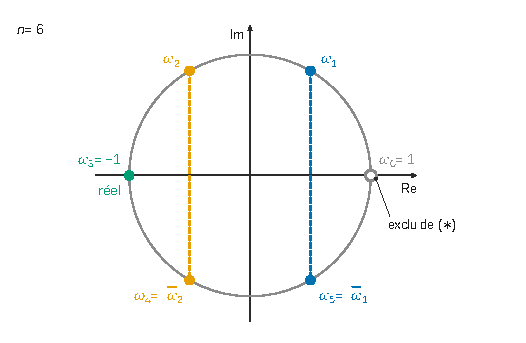
\includegraphics{figures/q9-racines-conjuguees.pdf}
\caption*{Figure 1 --- Cas n = 6 : ω\_0 = 1 est exclu du produit (∗), les autres
racines s'apparient en conjugués ω\_5 = ω̄\_1, ω\_4 = ω̄\_2, et ω\_3 = −1
est réel}
\end{figure}

\begin{methode}

Vérification directe : \(\overline{P(\omega_k)}=P(\overline{\omega_k})=P(\omega_{n-k})\) car \(P\) est réel, et \(k\mapsto n-k\) permute \([\![1,n-1]\!]\). Le produit est donc égal à son conjugué. Pour lever une hypothèse de non-annulation, la perturbation \(A+xI_n\) suivie d'un passage à la limite est un réflexe utile.

\end{methode}

\begin{piege}

Le raccourci « \(\det A\) réel, \(P(1)\) réel, donc le quotient est réel » oublie le cas \(P(1)=0\). Exemple : \(n=3\) et \(P=1+X-2X^2\), pour lequel le produit vaut \(9\).

\end{piege}

\begin{jury}

Rapport 2026 : la question n'a pas posé de problème quand les précédentes étaient faites, et « Quelques candidats se sont posés la question du cas où 1 était racine de \(P\) ». C'est bien la difficulté de la question : la traiter explicitement.

\end{jury}

\begin{center}\rule{0.5\linewidth}{0.5pt}\end{center}

\hypertarget{probluxe8me-polynuxf4mes-de-laguerre}{%
\section{Problème --- Polynômes de Laguerre}\label{probluxe8me-polynuxf4mes-de-laguerre}}

Le problème construit un espace préhilbertien de fonctions et y exhibe une famille orthonormale de polynômes. Les outils sont la projection orthogonale, l'intégrabilité par comparaison et l'intégration par parties sur \([0,+\infty[\).

\hypertarget{question-10}{%
\subsection{Question 10}\label{question-10}}

\begin{indication}{1}

a) Le vecteur candidat est donné : vérifier les deux propriétés qui caractérisent \(p_F(x)\) dans la définition de l'énoncé.

\end{indication}

\begin{indication}{2}

a) Il suffit que \(x-y\) soit orthogonal à chaque \(e_j\) ; dire pourquoi cela suffit. b) Penser au théorème de Pythagore, deux fois.

\end{indication}

\hypertarget{solution-9}{%
\subsubsection{Solution}\label{solution-9}}

On n'utilise que la définition de l'énoncé : \(p_F(x)\) est l'unique vecteur de \(F\) tel que \(x-p_F(x)\in F^\perp\).

\textbf{a)} Soit \(y=\sum_{i=0}^n\langle x\mid e_i\rangle e_i\), qui appartient à \(F\). Pour tout \(j\) :
\equationajustee{\begin{aligned}
\langle x-y\mid e_j\rangle&=\langle x\mid e_j\rangle-\sum_i\langle x\mid e_i\rangle\delta_{ij}\\
&=0.
\end{aligned}}
Donc \(x-y\) est orthogonal à la famille génératrice \((e_j)\) de \(F\), donc à \(F\) par linéarité : \(x-y\in F^\perp\). Par unicité :
\equationajustee{\boxed{p_F(x)=\sum_{i=0}^n\langle x\mid e_i\rangle e_i}}

\textbf{b)} \(p=p_F(x)\in F\) et \(x-p\in F^\perp\) sont orthogonaux. Par Pythagore :
\equationajustee{\begin{aligned}
\|x\|^2&=\|p\|^2+\|x-p\|^2\\
&\ge\|p\|^2.
\end{aligned}}
\equationajustee{\boxed{\|p_F(x)\|^2\le\|x\|^2}}
Et, \((e_i)\) étant orthonormale, \(\|p\|^2=\sum_i\langle x\mid e_i\rangle^2\) :
\equationajustee{\boxed{\sum_{i=0}^n\langle x\mid e_i\rangle^2\le\|x\|^2}}

\begin{figure}[H]
\centering
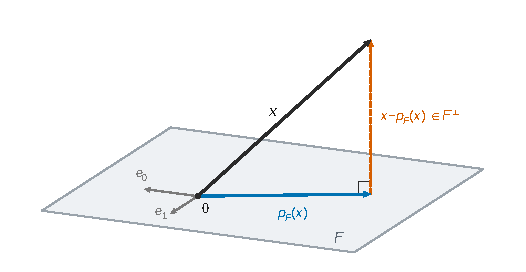
\includegraphics{figures/q10-projection-orthogonale.pdf}
\caption*{Figure 2 --- Projeté orthogonal : p\_F(x) ∈ F et x − p\_F(x) ∈ F⊥ sont
les côtés de l'angle droit d'un triangle rectangle d'hypoténuse x}
\end{figure}

\begin{piege}

Ne pas compléter \((e_0,\dots,e_n)\) en une base orthonormale de \(E\) : le rapport 2026 rappelle que « L'espace \(E\) n'étant pas de dimension finie \emph{a priori}, le théorème de la base incomplète ne s'applique pas ici. »

\end{piege}

\begin{jury}

Rapport 2026, Q10.a : « Rédaction très brouillonne. Peu de candidats ont réellement répondu à la question en se basant sur les hypothèses données dans l'énoncé. » Toutes les étapes sont attendues : orthogonalité à une famille génératrice qui entraîne l'orthogonalité au sous-espace, appel explicite à l'unicité, orthogonalité de \(p\) et \(x-p\) avant d'écrire Pythagore. Q10.b appelle la même remarque, avec un peu plus de réussite.

\end{jury}

\hypertarget{question-11}{%
\subsection{Question 11}\label{question-11}}

\begin{indication}{1}

Développer un carré bien choisi.

\end{indication}

\begin{indication}{2}

Majorer \(|f(t)g(t)|\mathrm e^{-t}\) par une fonction que la définition de \(E\) rend intégrable.

\end{indication}

\hypertarget{solution-10}{%
\subsubsection{Solution}\label{solution-10}}

Comme \(|a|^2=a^2\) et \(|b|^2=b^2\), l'inégalité \((|a|-|b|)^2\ge0\) donne \(a^2+b^2-2|a||b|\ge0\), d'où \(\boxed{|ab|\le\frac{a^2+b^2}2}\).

Pour \(f,g\in E\), \(t\mapsto f(t)g(t)\mathrm e^{-t}\) est continue sur \(I\), et :
\equationajustee{|f(t)g(t)|\mathrm e^{-t}\le\tfrac12\big(f(t)^2\mathrm e^{-t}+g(t)^2\mathrm e^{-t}\big).}
Le majorant est intégrable sur \(I\) : \textbf{\(t\mapsto f(t)g(t)\mathrm e^{-t}\) est intégrable sur \(I\).}

\begin{piege}

L'intégrabilité porte sur la valeur absolue : c'est \(|f g|\mathrm e^{-t}\) qu'il faut majorer. Le rapport 2026 note que « La manipulation de la valeur absolue est mal maîtrisée par beaucoup de candidats ».

\end{piege}

\begin{piege}

Erreur relevée par le rapport 2026 : « le produit de deux fonctions intégrables est intégrable ». C'est faux : \(t\mapsto1/\sqrt t\) est intégrable sur \(]0,1]\), pas son carré. C'est la domination par \(\frac12(f^2+g^2)\mathrm e^{-t}\) qui conclut.

\end{piege}

\hypertarget{question-12}{%
\subsection{Question 12}\label{question-12}}

\begin{indication}{1}

Montrer que \(E\) est un sous-espace vectoriel d'un espace vectoriel connu plutôt que de vérifier tous les axiomes.

\end{indication}

\begin{indication}{2}

Pour la stabilité, développer \((f+\lambda g)^2\) et utiliser Q11. Pour le caractère défini, quel théorème concerne les fonctions continues positives d'intégrale nulle ?

\end{indication}

\hypertarget{solution-11}{%
\subsubsection{Solution}\label{solution-11}}

\emph{Structure.} \(E\subset\mathcal C(I,\mathbb R)\) contient \(0\). Pour \(f,g\in E\) et \(\lambda\in\mathbb R\), \(f+\lambda g\) est continue, et :
\equationajustee{(f+\lambda g)^2\mathrm e^{-t}=f^2\mathrm e^{-t}+2\lambda fg\,\mathrm e^{-t}+\lambda^2g^2\mathrm e^{-t}.}
Ce membre est intégrable (définition de \(E\) et Q11). \textbf{\(E\) est un sous-espace vectoriel de \(\mathcal C(I,\mathbb R)\).}

\emph{Produit scalaire.} L'application \((f,g)\mapsto\int_0^{+\infty}fg\,\mathrm e^{-t}\) est bien définie : l'intégrale converge par Q11. Elle est symétrique et positive.

Linéarité à gauche : pour \(f_1,f_2,g\in E\) et \(\lambda\in\mathbb R\), les intégrales \(\langle f_1\mid g\rangle\) et \(\langle f_2\mid g\rangle\) convergent (Q11). La linéarité de l'intégrale sur les intégrales convergentes donne \(\langle f_1+\lambda f_2\mid g\rangle=\langle f_1\mid g\rangle+\lambda\langle f_2\mid g\rangle\). Avec la symétrie, l'application est bilinéaire.

Caractère défini : si \(\langle f\mid f\rangle=0\), la fonction \(f^2\mathrm e^{-t}\) est \textbf{continue}, positive, d'intégrale nulle sur \(I\), donc nulle. Et \(f=0\) car \(\mathrm e^{-t}>0\).

\textbf{C'est un produit scalaire sur \(E\).}

\begin{piege}

Pour la structure, il ne suffit pas de vérifier la continuité de \(f+\lambda g\) : l'intégrabilité de \((f+\lambda g)^2\mathrm e^{-t}\) fait partie de la définition de \(E\). Le rapport 2026 relève cette confusion chez de nombreux candidats.

\end{piege}

\begin{piege}

Le caractère défini repose sur la continuité de \(f\) : sans elle, une fonction nulle sauf en un point serait de « norme » nulle.

\end{piege}

\begin{jury}

Rapport 2026 : « la linéarité a souvent été affirmée sans justification de la convergence des différentes intégrales et le caractère défini a souvent été fait très approximativement avec l'absence du caractère continu de la fonction dans l'intégrale. » Le jury signale aussi des copies où la linéarité se réduit à l'additivité seule ou à l'homogénéité seule : traiter \(f_1+\lambda f_2\) couvre les deux.

\end{jury}

\hypertarget{question-13}{%
\subsection{Question 13}\label{question-13}}

\begin{indication}{1}

Il s'agit d'abord de montrer que toute fonction polynomiale est dans \(E\) : comparer \(P(t)^2\mathrm e^{-t}\) à une fonction de Riemann en \(+\infty\).

\end{indication}

\begin{indication}{2}

Une fois \(F\subset E\) acquis, quelle propriété de \(\mathbb R_n[X]\) lui-même suffit à conclure ?

\end{indication}

\hypertarget{solution-12}{%
\subsubsection{Solution}\label{solution-12}}

\emph{Inclusion.} Soit \(P\in\mathbb R_n[X]\). La fonction \(t\mapsto P(t)^2\mathrm e^{-t}\) est continue et positive sur \(I\).

Par croissances comparées, \(t^2P(t)^2\mathrm e^{-t}\to0\), donc \(P(t)^2\mathrm e^{-t}=o(1/t^2)\) en \(+\infty\). Elle est donc intégrable sur \([1,+\infty[\), et sur \([0,1]\) par continuité. Donc \(P\in E\).

\emph{Structure.} \(F\subset E\), et \(F=\mathbb R_n[X]\) est lui-même un espace vectoriel (il contient \(0\), il est stable par combinaison linéaire), pour les lois de \(E\). \textbf{\(F\) est un sous-espace vectoriel de \(E\).}

\(F\) est de dimension \(n+1\), car un polynôme nul sur l'ensemble infini \(I\) est nul. Cela justifie aussi que \(\langle\ \mid\ \rangle\) est défini positif sur \(\mathbb R[X]\).

\begin{methode}

Pour l'intégrabilité en \(+\infty\) d'un « polynôme fois exponentielle décroissante », la comparaison à \(1/t^2\) par un \(o\) est le réflexe standard.

\end{methode}

\begin{piege}

Un \(o\) n'est pas un équivalent. Le rapport 2026 cite l'équivalent faux « \(t^{2k}e^{-t}\) équivalent à \(e^{-\frac{t}{2}}\) en l'infini ».

Le quotient \(t^{2k}\mathrm e^{-t/2}\) tend vers \(0\), pas vers \(1\). On écrit \(t^{2k}\mathrm e^{-t}=o(\mathrm e^{-t/2})\) ou \(o(1/t^2)\).

\end{piege}

\begin{jury}

Rapport 2026 : « La question a été mal traitée en grande partie. Beaucoup de candidats ont soit oublié de démontrer que \(F\) était bien inclus dans \(E\), soit ont voulu démontrer que \(F\) était un sev de \(E\) en montrant l'appartenance à \(E\) de la combinaison linéaire d'éléments de \(F\). »

L'inclusion est le cœur de la question, et la stabilité se lit dans \(\mathbb R_n[X]\).

\end{jury}

\hypertarget{question-14}{%
\subsection{Question 14}\label{question-14}}

\begin{indication}{1}

a) Dérivée \(p\)-ième d'un produit : formule de Leibniz.

\end{indication}

\begin{indication}{2}

a) Pour \(p<n\), regarder l'exposant minimal de \(x\) dans chaque terme. b) Prendre \(p=n\) et simplifier le facteur exponentiel.

\end{indication}

\hypertarget{solution-13}{%
\subsubsection{Solution}\label{solution-13}}

\textbf{a)} On a \((x^n)^{(k)}=\frac{n!}{(n-k)!}x^{n-k}\) pour \(k\le n\), et \((\mathrm e^{-x})^{(m)}=(-1)^m\mathrm e^{-x}\). Pour \(p\le n\), Leibniz donne :
\equationajustee{\boxed{h_n^{(p)}(x)=\mathrm e^{-x}\sum_{k=0}^p(-1)^{p-k}\binom pk\frac{n!}{(n-k)!}x^{n-k}}}
Si \(p<n\), tous les exposants vérifient \(n-k\ge n-p\ge1\) : \(\boxed{h_n^{(p)}(0)=0}\).

\textbf{b)} Pour \(p=n\) :
\equationajustee{\begin{aligned}
L_n(x)&=\frac{\mathrm e^x}{n!}h_n^{(n)}(x)\\
&=\sum_{k=0}^n(-1)^{n-k}\binom nk\frac{x^{n-k}}{(n-k)!}.
\end{aligned}}
Avec \(m=n-k\) :
\equationajustee{\boxed{L_n=\sum_{m=0}^n(-1)^m\binom nm\frac{X^m}{m!}\in\mathbb R[X]}}
\equationajustee{\boxed{\deg L_n=n,\ \text{de coefficient dominant }\frac{(-1)^n}{n!}}}
Par exemple \(L_1=1-X\) et \(L_2=1-2X+\frac{X^2}2\).

\begin{methode}

Le rapport 2026 note que quelques candidats ont tenté une récurrence, « très souvent fausse et non aboutie », et qu'il y a eu peu d'erreurs avec Leibniz. Pour une dérivée \(p\)-ième d'un produit, Leibniz est l'outil direct.

\end{methode}

\begin{piege}

Préciser le degré impose de vérifier que le coefficient de \(X^n\) est non nul. Ne pas oublier le signe \((-1)^{p-k}\) venant de \(\mathrm e^{-x}\).

Et \(L_n\) est un polynôme parce que le facteur \(\mathrm e^{x}\) compense exactement le \(\mathrm e^{-x}\) de \(h_n^{(n)}\), pas parce que l'exponentielle serait un « polynôme de degré infini » (erreur relevée par le jury).

\end{piege}

\hypertarget{question-15}{%
\subsection{Question 15}\label{question-15}}

\begin{indication}{1}

Transférer les \(n\) dérivations de \(h_n\) sur \(g\) par intégrations par parties successives.

\end{indication}

\begin{indication}{2}

Travailler sur un segment \([0,A]\) ; les termes de bord en \(0\) sont réglés par Q14.a, ceux en \(A\) par croissances comparées. Écrire une récurrence propre sur le nombre d'intégrations par parties.

\end{indication}

\begin{indication}{3}

Relire attentivement la définition du crochet de Q12 : avec ou sans le poids \(\mathrm e^{-t}\), la première formule demandée est-elle cohérente ?

\end{indication}

\hypertarget{solution-14}{%
\subsubsection{Solution}\label{solution-14}}

\emph{Défaut d'énoncé.} Avec le poids de Q12, \(\langle g\mid h_n^{(n)}\rangle=\int_0^{+\infty}g\,h_n^{(n)}\mathrm e^{-t}\) ne s'exprime pas à l'aide de \(\int_0^{+\infty}g^{(n)}h_n\). Pour \(n=1\) et \(g=1\), le premier vaut \(\int_0^{+\infty}(1-t)\mathrm e^{-2t}\,\mathrm dt=\frac14\), le second \(0\).

On exprime donc l'intégrale sans poids \(\int_0^{+\infty}g(t)h_n^{(n)}(t)\,\mathrm dt\) en fonction de \(\int_0^{+\infty}g^{(n)}(t)h_n(t)\,\mathrm dt\). C'est la formulation corrigée que donne le rapport 2026. Cette intégrale vaut \(n!\,\langle g\mid L_n\rangle\) car \(h_n^{(n)}=n!\,L_n\mathrm e^{-t}\) : le poids est déjà dans \(h_n^{(n)}\).

Soit \(g\in\mathbb R[X]\). Toutes les fonctions \(g^{(p)}h_n^{(q)}\) sont de la forme \(R(t)\mathrm e^{-t}\), avec \(R\) polynomiale (Q14.a). Elles sont donc intégrables sur \(I\).

Montrons par récurrence sur \(p\in[\![0,n]\!]\) :
\equationajustee{\int_0^{+\infty}g\,h_n^{(n)}=(-1)^p\int_0^{+\infty}g^{(p)}h_n^{(n-p)}.}
Le cas \(p=0\) est clair. Pour \(p\le n-1\), sur \([0,A]\) :
\equationajustee{\int_0^Ag^{(p)}h_n^{(n-p)}=\Big[g^{(p)}h_n^{(n-p-1)}\Big]_0^A-\int_0^Ag^{(p+1)}h_n^{(n-p-1)}.}
Le crochet est nul en \(0\) (Q14.a, car \(n-p-1<n\)).

En \(A\), il est de la forme \(R(A)\mathrm e^{-A}\), qui tend vers \(0\). Les intégrales convergeant, on passe à la limite et l'on obtient le rang \(p+1\). Pour \(p=n\) :
\equationajustee{\boxed{\int_0^{+\infty}g(t)h_n^{(n)}(t)\,\mathrm dt=(-1)^n\int_0^{+\infty}g^{(n)}(t)h_n(t)\,\mathrm dt}}
\equationajustee{\boxed{\langle g\mid L_n\rangle=\frac{(-1)^n}{n!}\int_0^{+\infty}g^{(n)}(t)\,t^n\mathrm e^{-t}\,\mathrm dt}}

\begin{methode}

Intégration par parties sur un intervalle non borné : on la fait sur \([0,A]\), on justifie la convergence des intégrales et la limite du crochet, puis on fait tendre \(A\) vers \(+\infty\).

\end{methode}

\begin{jury}

Rapport 2026 : l'énoncé comportait une erreur, la première demande devant porter sur \(\int_0^{+\infty}g(t)h_n^{(n)}(t)\,\mathrm dt\). « Les correcteurs auront fait preuve de bienveillance dans leur correction. Le barème a été adapté. » Le jury note des tentatives infructueuses sur la partie erronée, peu de bonnes tentatives sur la seconde, et des candidats qui ont réussi la question « en laissant de côté la première égalité à démontrer ». Signaler l'incohérence et poursuivre est la bonne stratégie.

\end{jury}

\hypertarget{question-16}{%
\subsection{Question 16}\label{question-16}}

\begin{indication}{1}

Appliquer Q15 avec le polynôme de plus petit degré dans le rôle de \(g\).

\end{indication}

\hypertarget{solution-15}{%
\subsubsection{Solution}\label{solution-15}}

Pour \(i<j\), Q15 avec \(g=L_i\) et l'indice \(j\) donne :
\equationajustee{\langle L_i\mid L_j\rangle=\frac{(-1)^j}{j!}\int_0^{+\infty}L_i^{(j)}(t)\,t^j\mathrm e^{-t}\,\mathrm dt.}
Or \(L_i^{(j)}=0\) car \(\deg L_i=i<j\) :
\equationajustee{\boxed{\langle L_i\mid L_j\rangle=0}}

\begin{piege}

C'est l'indice le plus grand qui doit fournir les dérivations : avec \(g=L_j\) et l'indice \(i\), on obtient \(L_j^{(i)}\neq0\) et l'argument ne conclut pas.

\end{piege}

\begin{jury}

Rapport 2026 : « Peu de réussite. Certains candidats ont pressenti le résultat et ont essayé de passer en force en donnant une intégrale qui visiblement n'était pas convergente et dont ils affirmaient qu'elle était nulle. » Toute intégrale écrite doit être convergente : ici, celle de Q15 l'est, et son intégrande est nul.

\end{jury}

\hypertarget{question-17}{%
\subsection{Question 17}\label{question-17}}

\begin{indication}{1}

Une intégration par parties relie \(\int t^n\mathrm e^{-t}\) à \(\int t^{n-1}\mathrm e^{-t}\).

\end{indication}

\begin{indication}{2}

Pour \(\langle L_n\mid L_n\rangle\), appliquer Q15 avec \(g=L_n\) : que vaut la dérivée \(n\)-ième d'un polynôme de degré \(n\) ?

\end{indication}

\hypertarget{solution-16}{%
\subsubsection{Solution}\label{solution-16}}

Soit \(I_n=\int_0^{+\infty}t^n\mathrm e^{-t}\,\mathrm dt\).

\emph{Existence.} L'intégrande est continu et positif sur \(I\), et \(t^{n+2}\mathrm e^{-t}\to0\) en \(+\infty\) : \(t^n\mathrm e^{-t}=o(1/t^2)\), donc \(I_n\) converge.

\emph{Calcul.} \(I_0=1\). Pour \(n\ge1\) :
\equationajustee{\int_0^At^n\mathrm e^{-t}\,\mathrm dt=-A^n\mathrm e^{-A}+n\int_0^At^{n-1}\mathrm e^{-t}\,\mathrm dt.}
Comme \(A^n\mathrm e^{-A}\to0\), on obtient \(I_n=nI_{n-1}\), et par récurrence :
\equationajustee{\boxed{\int_0^{+\infty}t^n\mathrm e^{-t}\,\mathrm dt=n!}}
\(L_n^{(n)}=n!\times\frac{(-1)^n}{n!}=(-1)^n\). Donc par Q15 :
\equationajustee{\langle L_n\mid L_n\rangle=\frac{(-1)^n}{n!}(-1)^nI_n.}
\equationajustee{\boxed{\langle L_n\mid L_n\rangle=1}}

\begin{piege}

La dérivée \(n\)-ième de \(cX^n\) vaut \(c\,n!\), pas \(c\). Contrôle : \(\langle L_0\mid L_0\rangle=\int_0^{+\infty}\mathrm e^{-t}\,\mathrm dt=1\).

\end{piege}

\begin{jury}

Rapport 2026 : « L'existence et le calcul de l'intégrale ont rarement été justifiés parfaitement ». Deux lignes suffisent : la convergence par comparaison, puis la limite du crochet \(A^n\mathrm e^{-A}\) avant de passer à la limite dans l'intégration par parties.

\end{jury}

\hypertarget{question-18}{%
\subsection{Question 18}\label{question-18}}

\begin{indication}{1}

Une famille orthonormale est libre. Combien de vecteurs, dans quel espace ?

\end{indication}

\begin{indication}{2}

Pour le projeté, la question de cours s'applique telle quelle.

\end{indication}

\hypertarget{solution-17}{%
\subsubsection{Solution}\label{solution-17}}

\((L_0,\dots,L_n)\) est une famille de \(F\) (Q14.b), orthonormale (Q16, Q17), donc libre. Elle est de cardinal \(n+1=\dim F\) (Q13) :
\equationajustee{\boxed{(L_0,\dots,L_n)\text{ est une base orthonormale de }F}}
Par Q10.a, pour tout \(g\in E\) :
\equationajustee{\boxed{p_F(g)=\sum_{k=0}^n\langle g\mid L_k\rangle L_k}}

\begin{jury}

Rapport 2026 : question bien faite par ceux qui avaient réussi les précédentes, mais « Certains ont admis les résultats (non démontrés) pour conclure sur la famille des \(L_i\) ». Admettre Q16 ou Q17 est permis à condition de le dire explicitement.

\end{jury}

\hypertarget{question-19}{%
\subsection{Question 19}\label{question-19}}

\begin{indication}{1}

Appliquer l'inégalité de Q10.b pour chaque entier \(N\), avec un sous-espace bien choisi.

\end{indication}

\begin{indication}{2}

Une série à termes positifs dont les sommes partielles sont majorées converge.

\end{indication}

\hypertarget{solution-18}{%
\subsubsection{Solution}\label{solution-18}}

Soient \(g\in E\) et \(N\in\mathbb N\). La famille \((L_0,\dots,L_N)\) est une base orthonormale de \(\mathbb R_N[X]\) (Q18 avec \(N\) à la place de \(n\)). Q10.b donne :
\equationajustee{\sum_{k=0}^N\langle g\mid L_k\rangle^2\le\|g\|^2.}
La série \(\sum\langle g\mid L_n\rangle^2\) est à termes positifs, et ses sommes partielles sont majorées par \(\|g\|^2\), indépendant de \(N\). Elle converge, et :
\equationajustee{\boxed{\sum_{n=0}^{+\infty}\langle g\mid L_n\rangle^2\le\|g\|^2}}
avec \(\|g\|^2=\int_0^{+\infty}g(t)^2\mathrm e^{-t}\,\mathrm dt\).

\begin{piege}

Ne pas passer à la limite dans l'inégalité avant d'avoir établi la convergence. Le rapport 2026 relève ce défaut : les candidats « passent à la limite pour dire ensuite que la limite existe ». L'ordre est : termes positifs, sommes partielles majorées, donc convergence, puis seulement passage à la limite.

\end{piege}

\begin{piege}

Ne pas invoquer une égalité de Parseval : elle n'est pas établie dans ce cadre, et c'est l'objet de Q20 d'en vérifier un cas.

\end{piege}

\hypertarget{question-20}{%
\subsection{Question 20}\label{question-20}}

\begin{indication}{1}

Pour l'appartenance à \(E\), calculer \(g_\alpha(t)^2\mathrm e^{-t}\) et discuter selon \(\alpha\) : l'énoncé dit-il vrai pour tout \(\alpha\) réel ?

\end{indication}

\begin{indication}{2}

Pour \(\langle g_\alpha\mid L_n\rangle\), développer \(L_n\) sur la base canonique (somme finie) et calculer \(\int_0^{+\infty}t^m\mathrm e^{-\beta t}\,\mathrm dt\) par changement de variable et Q17.

\end{indication}

\begin{indication}{3}

Le binôme fait apparaître une puissance \(n\)-ième ; la somme des carrés est alors une série géométrique dont il faut vérifier la raison.

\end{indication}

\hypertarget{solution-19}{%
\subsubsection{Solution}\label{solution-19}}

\emph{Défaut d'énoncé.} « Pour tout \(\alpha\in\mathbb R\), \(g_\alpha\in E\) » est faux. On montre l'équivalence avec \(\alpha>-\frac12\), hypothèse posée en tête de la question.

\(g_\alpha\) est continue et \(g_\alpha^2\mathrm e^{-t}=\mathrm e^{-(2\alpha+1)t}\). Cette fonction est intégrable sur \([0,+\infty[\) si et seulement si \(2\alpha+1>0\) (sinon elle est minorée par \(1\)) :
\equationajustee{\boxed{g_\alpha\in E\iff\alpha>-\tfrac12}}
\equationajustee{\boxed{\|g_\alpha\|^2=\frac1{2\alpha+1}}}

Soit \(\alpha>-\frac12\) et \(\beta=\alpha+1>0\). Par le changement de variable \(u=\beta t\) et Q17, \(\int_0^{+\infty}t^m\mathrm e^{-\beta t}\,\mathrm dt=\frac{m!}{\beta^{m+1}}\). Par linéarité (somme finie) :
\equationajustee{\begin{aligned}
\langle g_\alpha\mid L_n\rangle&=\sum_{m=0}^n(-1)^m\binom nm\frac1{m!}\cdot\frac{m!}{\beta^{m+1}}\\
&=\frac1\beta\Big(1-\frac1\beta\Big)^n.
\end{aligned}}
\equationajustee{\boxed{\langle g_\alpha\mid L_n\rangle=\frac{\alpha^n}{(\alpha+1)^{n+1}}}}

Soit \(q=\frac\alpha{\alpha+1}\). Comme \(\alpha+1>0\) :
\equationajustee{\begin{aligned}
|q|<1&\iff-(\alpha+1)<\alpha<\alpha+1\\
&\iff\alpha>-\tfrac12.
\end{aligned}}
Donc la série géométrique de raison \(q^2\) converge, et :
\equationajustee{\begin{aligned}
\sum_{n=0}^{+\infty}\langle g_\alpha\mid L_n\rangle^2&=\frac1{(\alpha+1)^2}\cdot\frac1{1-q^2}\\
&=\frac1{(\alpha+1)^2-\alpha^2}\\
&=\frac1{2\alpha+1}.
\end{aligned}}
\equationajustee{\boxed{\sum_{n=0}^{+\infty}\langle g_\alpha\mid L_n\rangle^2=\|g_\alpha\|^2}}
L'inégalité de Bessel de Q19 est une égalité pour les \(g_\alpha\). Contrôle : pour \(\alpha=0\), \(g_0=1=L_0\), les coefficients valent \(1,0,0,\dots\) et la somme vaut \(1=\|g_0\|^2\).

\begin{methode}

Q15 n'a été établie que pour \(g\) polynomiale. On peut l'étendre à \(g_\alpha\) (les termes de bord sont de la forme \(R(A)\mathrm e^{-\beta A}\to0\) car \(\beta>0\)), mais il faut l'écrire ; le développement de \(L_n\) sur la base canonique évite cette vérification.

\end{methode}

\begin{piege}

La condition \(|q|<1\) n'est pas décorative : elle équivaut exactement à \(\alpha>-\frac12\), la même condition que l'appartenance à \(E\).

\end{piege}

\begin{jury}

Rapport 2026 : « L'appartenance à \(E\) a généralement été bien traitée. La 2e partie de la question a été rarement abordée. » Le calcul des coefficients est pourtant accessible avec Q14.b et Q17 seulement : il rapporte des points même si Q15 n'a pas été faite.

\end{jury}

\begin{center}\rule{0.5\linewidth}{0.5pt}\end{center}

\hypertarget{bilan}{%
\section{Bilan}\label{bilan}}

\textbf{Ce que le rapport 2026 met en avant.} Moyenne 10,18, écart-type 4,51. Les exercices ont été le terrain de l'algèbre linéaire « sans calcul » : il faut nommer le théorème qui donne la diagonalisabilité (Q1, Q8) et le caractère scindé à racines simples (Q3).

Le début du problème (Q10, Q12, Q13), pourtant proche du cours, a coûté cher : rédaction fondée sur les seules hypothèses de l'énoncé, convergence de chaque intégrale avant toute linéarité, inclusion \(F\subset E\). Q4.a, Q16, Q19 et la fin de Q20 ont été rarement réussies. En conclusion, le jury demande de citer tous les théorèmes utilisés avec leurs hypothèses, d'utiliser chaque hypothèse en disant où elle sert, et de ne pas essayer « d'escroquer » les correcteurs en « trafiquant les calculs ».

\textbf{Méthodes à retenir.}

\begin{itemize}
\tightlist
\item
  Polynôme annulateur scindé à racines simples pour diagonaliser sans déterminant ; polynôme minimal d'une matrice diagonalisable = produit des \(X-\lambda\) sur les valeurs propres distinctes.
\item
  Puissances d'une matrice : reste de la division euclidienne par un polynôme annulateur (évaluation aux racines), ou binôme quand \(A=\alpha N+\beta I\) avec \(N\) simple.
\item
  Matrices circulantes : \(A=P(J)\), diagonalisées par la base de Fourier \(V_k={}^t(1,\omega_k,\dots,\omega_k^{n-1})\), de valeurs propres \(P(\omega_k)\).
\item
  Lever une hypothèse de non-annulation par perturbation (\(A+xI_n\)) et continuité.
\item
  Espaces de fonctions de carré intégrable pour un poids : stabilité par \(|ab|\le\frac{a^2+b^2}2\), caractère défini par continuité.
\item
  Formule de Rodrigues et intégrations par parties répétées pour établir l'orthogonalité d'une famille de polynômes ; termes de bord traités sur un segment puis à la limite.
\item
  Inégalité de Bessel : sommes partielles majorées, série à termes positifs, convergence avant passage à la limite.
\end{itemize}

\textbf{Prérequis à revoir.} Critères de diagonalisabilité, polynôme minimal, développement d'un déterminant, racines de l'unité ; intégrabilité sur un intervalle non borné, comparaison par \(o\) (et non par un équivalent faux), \(\int_0^{+\infty}t^n\mathrm e^{-t}\,\mathrm dt=n!\), formule de Leibniz, projection orthogonale.

\textbf{Questions classiques transposables.} Matrice « tout à 1 » et ses puissances ; déterminant circulant \(\prod_kP(\omega_k)\) ; orthogonalité des polynômes de Legendre, Hermite ou Tchebychev par la même technique (formule de Rodrigues et intégrations par parties) ; calcul de coefficients dans une base orthonormale par la formule du binôme et une série géométrique.

\end{document}
